\beginsong{Leise weht der Wind}[
    wuw={von einer Großfahrt des BdP ins Belledonne-Massiv}, 
    jahr={1983}, 
    bo={228}, 
    pfii={92}, 
    pfiii={28}, 
    gruen={30}, 
    kssiv={8}, 
    siru={157},
]

\beginverse
\endverse
\centering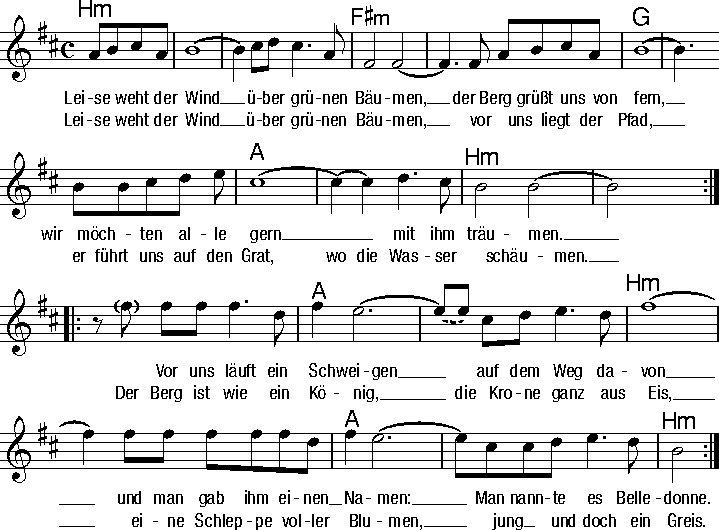
\includegraphics[width=1\textwidth]{Noten/Lied062.pdf}	

\beginverse
\[Hm]Leise weht der Wind über kahlen \[F#m]Steinen,
ein letzter Blick zu\[G]rück, dort liegt nicht das \[A]Glück,
das wir \[Hm]meinen.
Leise weht der Wind über kahlen \[F#m]Steinen,
nur wer den Berg ver\[G]steht, auf den Gipfel \[A]geht,
denn Grenzen gibt es \[Hm]keine.
\endverse

\beginchorus
Vor uns läuft ein \[A]Schweigen auf dem Weg da\[Hm]von
und man gab ihm einen Na\[A]men:
Man nannte es Belle\[Hm]donne.
Der Berg ist wie ein Kö\[A]nig, die Krone ganz aus \[Hm]Eis,
eine Schleppe voller Blu\[A]men, jung und doch ein \[Hm]Greis.
\endchorus

\beginverse
^Leise weht der Wind über Gletscher^seen.
Wie weit werden wir noch ^kommen? Die Kraft ist uns ge^nommen,
doch die Fahrt muss weiter ^gehen.
Leise weht der Wind über Gletscher^seen.
Unser Ziel erreicht, wir ^scherzen, vergessen alle ^Schmerzen,
wenn wir über allem ^stehen.
\endverse

\printchorus

\beginverse
^Leise weht der Wind über's Alltags^leben,
vor uns liegt die ^Stadt, die keine Seele ^hat.
Was ist der Berg da^gegen?
Leise weht der Wind über's Alltags^leben,
ab und zu dreh'n wir uns ^um, doch die Gipfel bleiben ^stumm,
wir möchten gern' mit ihnen ^reden.
\endverse

\beginchorus
Vor uns liegt die \[A]Eile der Zivilisa\[Hm]tion,
doch wir kehren wie\[A]der
zu uns'rem Freund Belle\[Hm]donne.
Er ist wie ein Kö\[A]nig, die Krone ganz aus \[Hm]Eis,
eine Schleppe voller Blu\[A]men und der Wind weht \[Hm]leis'.
\endchorus

\endsong

\beginscripture{}
Das Belledonne-Massiv ist ein 60 km langer Ausläufer der Alpen in Ostfrankreich, das bis in 2.980m Höhe reicht.
\endscripture
